% THIS IS AN EXAMPLE DOCUMENT FOR VLDB 2012
% based on ACM SIGPROC-SP.TEX VERSION 2.7
% Modified by  Gerald Weber <gerald@cs.auckland.ac.nz>
% Removed the requirement to include *bbl file in here. (AhmetSacan, Sep2012)
% Fixed the equation on page 3 to prevent line overflow. (AhmetSacan, Sep2012)

\documentclass{vldb}
\usepackage{graphicx}
\usepackage{balance}  % for  \balance command ON LAST PAGE  (only there!)
\usepackage{cases}
\usepackage{listings}
\usepackage{color}
\usepackage{algorithmicx}
\usepackage[]{algorithm}
%\usepackage[]{algorithm2e}
\usepackage{algpseudocode}
\usepackage{enumitem}
\usepackage{multicol}
%\usepackage{blindtext}
\usepackage{float}




\newcommand{\ceg}[1]{{\textcolor{green}{#1 --- CEG}}}
\newcommand{\eat}[1]{{}}

\begin{document}

% ****************** TITLE ****************************************

\title{Question Answering over a Probabilistic Knowledge Base}

% possible, but not really needed or used for PVLDB:
%\subtitle{[Extended Abstract]
%\titlenote{A full version of this paper is available as\textit{Author's Guide to Preparing ACM SIG Proceedings Using \LaTeX$2_\epsilon$\ and BibTeX} at \texttt{www.acm.org/eaddress.htm}}}

% ****************** AUTHORS **************************************

% You need the command \numberofauthors to handle the 'placement
% and alignment' of the authors beneath the title.
%
% For aesthetic reasons, we recommend 'three authors at a time'
% i.e. three 'name/affiliation blocks' be placed beneath the title.
%
% NOTE: You are NOT restricted in how many 'rows' of
% "name/affiliations" may appear. We just ask that you restrict
% the number of 'columns' to three.
%
% Because of the available 'opening page real-estate'
% we ask you to refrain from putting more than six authors
% (two rows with three columns) beneath the article title.
% More than six makes the first-page appear very cluttered indeed.
%
% Use the \alignauthor commands to handle the names
% and affiliations for an 'aesthetic maximum' of six authors.
% Add names, affiliations, addresses for
% the seventh etc. author(s) as the argument for the
% \additionalauthors command.
% These 'additional authors' will be output/set for you
% without further effort on your part as the last section in
% the body of your article BEFORE References or any Appendices.


\author{\alignauthor Christan Grant, Kun Li, Yan Chen, Daisy Zhe Wang\\
       \affaddr{University of Florida}\\
       \affaddr{Computer \& Information Science \& Engineering Department}\\
       \affaddr{Gainesville, Florida}\\
       \email{\{cgrant,kli,yang,daisyw\} @ cise.ufl.edu}
}


\maketitle



\begin{abstract}

As knowledge bases gain appeal from large companies and organizations,
the high volatility of facts is making \emph{probabilistic} knowledge bases,
knowledge bases with uncertainty attached to each fact, the next frontier.
In this demonstration, we a present question answering application over large probabilistic knowledge bases.
This demonstration allows attendees to interact with three large
probabilistic knowledge bases, one with primarily deterministic rules, 
another with a large amount of rules extracted from the web, and a third from a
continuously learning system.
In addition, the use of a probabilistic knowledge base allows the system to
quantify the truthfulness of evaluated questions by computing the joint
probabilities of facts that support the answer to each questions.
We leverage a popular question answering system for language translation and we perform all
knowledge base computations--including, grounding and inference--inside the
PostgreSQL Relational Database Management System.
We believe this demonstration to be the first to demonstrate such an
application over probabilistic knowledge bases.


\end{abstract}




\section{Introduction}

%Motivate Prob KBs
%Describe Motivation of the the KHop system.
%Give example scenario.
%Introduce the Khop system.
%Describe intro that this demo show real time incremental changes and probability changes to a large KB.

In recent years, the large increase of machine accessible data has lead researchers
to develop sophisticated methods of organizing and using the information.
In particular, the advancement of information extraction techniques has allowed
millions of facts to be extracted from across the web.
This is evidenced by the renewed interests in knowledge graphs and knowledge bases
from companies and
researchers~\cite{bellare2013woo,chang2014typed,dong2014knowledge,niu2012deepdive}.

Knowledge graphs efficiently store and manage the linking of facts.
Knowledge bases are equivalent to knowledge graphs but with and additional
inference engine. 
Inference engines allow the discovery of facts that are not explicitly
mentioned in the knowledge graph.
Researchers currently pair probabilities with extracted facts and rules to
represent the natural uncertainty found in language and extraction systems.
These stores are called probabilistic knowledge bases~\cite{chen2014knowledge}.
When performing inference, probabilistic knowledge bases consider the uncertainty
of facts upon evaluation.

This demonstration describes a question answering application developed to demonstrate
a new probabilistic knowledge base begin developed in the data science research group at the University of Florida.
Attendees will gain an understanding of the usefulness of a probabilistic
knowledge base and the techniques developed for large-scale knowledge base
management.
The question answering application allows users to see example queries to a
probabilistic knowledge base and also to understand how probabilistic knowledge bases work in general.

Further, we enumerate our contributions as follows:
\begin{itemize}
\vspace{-0.5em}
\item We develop a question answering architecture that leverages a probabilistic knowledge base for answer generation.

\vspace{-0.5em}
\item We develop a trustworthiness value for each question answered over three difference knowledge bases.

\vspace{-0.5em}
\item We describe an application for users to interact with a probabilistic knowledge
base. Users can add and removing facts before to recompute answer
trustworthiness.
\end{itemize}

\begin{figure}
%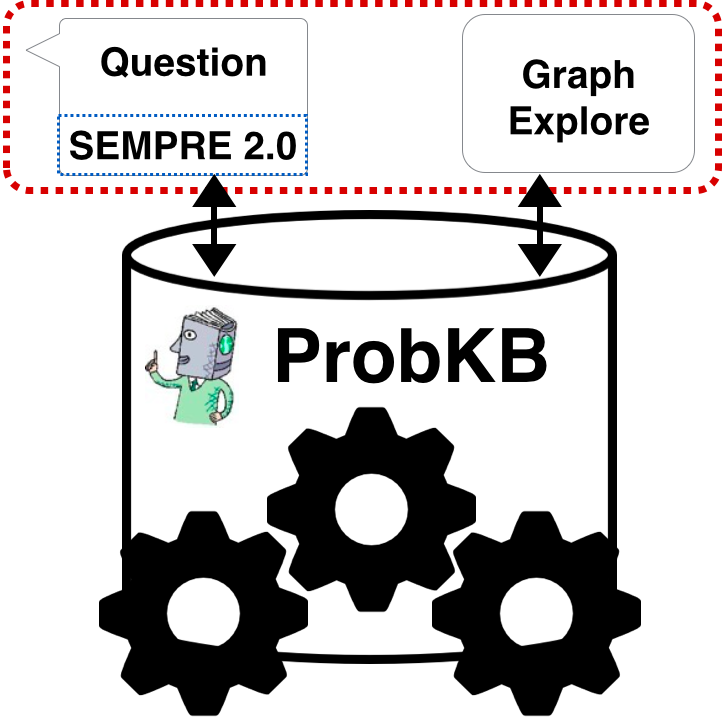
\includegraphics[width=\columnwidth,clip=true,trim=0cm 4cm 0cm 10cm]{images/qaarchitecture.png}
\centering
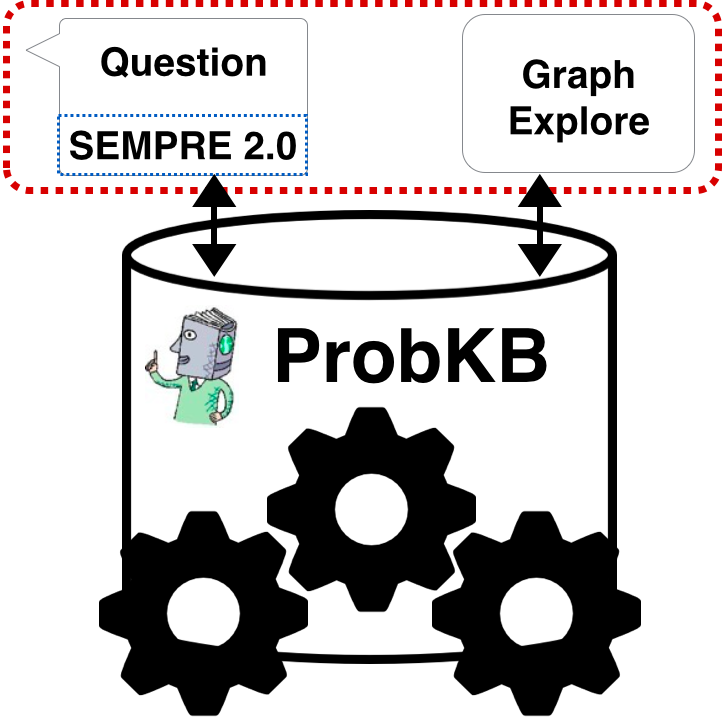
\includegraphics[width=0.6\columnwidth]{images/probqa-architecture.png}
\caption{Question answering system architecture.}
\label{fig:qaarchitecture}
\end{figure}




\section{Background}

In this section, we give the necessary background from the probabilistic knowledge base backed question answering system.
We first describe the set of data sets that underly this work.
We then give a brief description of Markov Logic Networks followed by our definition of a probabilistic knowledgebase.

\subsection{Data Set}
\label{sec:probqa-dataset}

In this demo, we use Freebase, Reverb, and NELL as the underlying knowledge bases.
These knowledge bases store collection of facts as (subject, predicate, object) triples,
representing facts related to real-world entities (people, places, and things).
Each knowledge base differs in scale, schema and construction methods.

\textbf{Freebase.} Freebase is a web-scale, human-crafted, high precision knowledge base of
well-known topics (entities) and facts~\cite{bollacker2008freebase}.
As of current writing, it contains 47.5 million entities
and 2.9 billion facts, spanning a variety of areas including People, Sports, Music, Internet,
Books, etc, organized into domains. The Freebase KB is publicly accessible as RDF triples.

\textbf{ReVerb.} ReVerb is an automatic knowledge base construction system
that extracts entities and facts from natural language text~\cite{fader2011identifying}.
It is a universal schema extraction system, extracting both entities and predicates (relations).
The extracted tuples are publicly available, and we use
its ClueWeb extractions, which contains 14.7 million facts, annotated by their confidence
and source URLs.

\textbf{NELL.} NELL is a never-ending knowledge extraction system~\cite{mitchell2015never}.
It extracts facts and updates its knowledge base every day.
As of current writing, it has extracted 84.6 million facts, of
which 2.2 million are believed to have high confidence.
Like ReVerb, each fact is annotated by its confidence and source URLs.
It also contains information on which extraction
algorithms are used to extract each fact.

In both ReVerb and NELL KBs, recent works have tried to mine \emph{first-order inference rules}.
An inference rule states causal relationships among facts, for example, we have
\[
\text{bornIn}(x, y), \text{locatedIn}(y, z) \rightarrow \text{bornIn}(x, z).
\]
This rule states that if a person \(x\) was born in location \(y\), and location \(y\)
is located within another location \(z\), then person \(x\) is also born in location \(z\).
The Sherlock-Holmes system~\cite{schoenmackers2010learning} mines 30,912 inference rules from ReVerb, and NELL also
has 2 thousand rules with an inference engine as one of its extraction component.


\subsection{Markov Logic Networks}

Markov Logic Networks (MLNs) are the standard method of modeling uncertainty.
MLNs are mare up of a weighted first-order formulae of the form \(\{F_i, W_i\}\),
where \(F_i\) is a logical expression and \(W_i\) is a weight
specifying how likely it is that the formula is true.

For example, the MLN clauses below state two different sets of information.

%\vspace{-1em}
%\begin{table}[h]
\noindent\begin{tabular}{l l}
  \(0.96\) & bornInState (Obama, Hawaii) \\
  \(1.40\) & \( \forall x \in Person, \forall y \in State, \forall z \in Country: \) \\
           & \(bornState(x,y) \wedge isState(y,z) \rightarrow bornCountry(x, z)\)
\end{tabular}
%\end{table}
%\vspace{-1em}

The first clause states that that Obama was born in the state of Hawaii.
The second formulate is an inference rule that states that if a person \(x\) is born in a state \(y\), and a state \(y\) is in a part of a country \(z\),
then that person \(x\) is born in the country \(z\).
These formula do not necessitate that the formula apply.
The weights of 0.96 and 1.40 specify the strength of the formula; stronger rules have a lower chance of being violated.
Deterministic rules, or rules that can never be violated are given an infinite weights of \(\infty\).


\subsubsection{Grounding}

MLNs are a template generating ground factor graphs.
A factor graph is a set of factors \(\Phi = \{ \phi_1, \ldots, \phi_{|\Phi|} \} \),
where each factor \(\phi_i\) is a function \(\phi_i (\mathbf{X}_i)\) over a
vector of random variables \(\mathbf{X}_i\).
%\ceg{Maybe add figure of ground factor graph}
The random variables correspond to facts (\(F_i\)) and factors a correspond to rules.

We use the term grounding to refer to the processes of creating the factor graph from an
MLN and a set of clauses.
Each node in the factor graph is a ground atom and has a boolean variable that represents its truth value.
We an perform the grounding step inside the database using a simple series of database queries~\cite{chen2014knowledge}.

For each possible grounding of formula \(F_i\) we create a ground factor
\(\phi_i(\mathbf{X}_i)\) with a value of 1 if the grounding is true, otherwise
\(e^{W_i}\). The marginal probability distribution of a set of grounded atoms \(\mathbf{X}\) is defined as
\begin{equation}
\label{eq:probqa-marginal}
P(\mathbf{X} = x) = \frac{1}{Z} \prod_i \phi_i (\mathbf{X}_i) = \frac{1}{Z} \text{exp} \left( \sum_i W_i n_i(x) \right),
\end{equation}
where \(n_i(x)\) is the number of true groundings of rule \(F_i\) in x, \(W_i\) is its weight, and \(Z\) is the partition function.
This probability gives use the probability of one particular state of a knowledge base.


%\subsubsection{Rule Generation}



%\subsubsection{Inference}


\subsection{Probabilistic Knowledge Bases}

We use a definition of probabilistic knowledge bases derived in previous work~\cite{chen2014knowledge}.
A probabilistic knowledge base is a 5-tuples \(\Gamma = (\mathcal{E}, \mathcal{C}, \mathcal{R}, \Pi, \mathcal{L})\), where
\begin{enumerate}[leftmargin=0cm,itemindent=.5cm,labelwidth=\itemindent,labelsep=0cm,align=left]
\vspace{-1em}
\item \(\mathcal{E} = \{ e_1, \ldots, e_{|\mathcal{E}|} \} \) is the set of entities.
Each entitie \( e \in \mathcal{E} \) refers to a real-world object.

\vspace{-1em}
\item \(\mathcal{C} = \{ c_1, \ldots, c_{|\mathcal{C}|} \} \) is the set of classes (or types).
Each class \( C \in \mathcal{C} \) maybe be a subset of \(\mathcal{E} : C \subseteq \mathcal{E}\), or an unknown class.

\vspace{-1em}
\item \(\mathcal{R} = \{ R_1, \ldots, R_{|\mathcal{R}|} \} \) is the set of relations.
Each \(R \in \mathcal{R} \) defines a binary relation on \(C_i, C_j \in \mathcal{C}: R: \subseteq C_i \times C_j\).
We call \(C_i, C_j\) the domain and range of \(R\) and use \(R(C_i,C_j)\) to denote the relation and its domain and range.


\vspace{-1em}
\item \(\Pi = \{(r_1, w_1), \ldots, (r_{|\Pi|}, w_{\Pi|})\} \) is a set of weighted facts.
For each \( (r,w) \in \Pi\), \(r\) is a tuple  \((R,x,y)\),
where \(R(C_i,C_j) \in \mathcal{R}, x \in C_i \in C, y \in C_j \in C\), and \((x,y) \in R\);
\(w \in \mathbb{R}\) is a weight indicating how likely it is that \(r\) is true. 

\vspace{-1em}
\item \(\mathcal{L} = \{(F_1,W_1),\ldots, (F_{|\mathcal{L}|}, W_{|\mathcal{L}|}) \} \) is a set of weighted rules.
For each \((F, W) \in \mathcal{L} \), \(F\) is a first-order logic clause, and
\(W \in \mathbb{R} \) us a weight indicating how likely the formula \(F\)
holds. 

\end{enumerate}


\subsubsection{Question Answering}

To answer questions, a mapping must be developed between a known
natural language utterance and a subset of all possible facts.
We assume that the knowledge base contains that complete set of facts necessary
to find the answer to the question.
Additionally, in order to quantify the truthfulness of each fact, it is
important to enumerate the facts that support the final answer.


In this work, we leverage a question answering system named SEMPRE which uses supervised
learning of question answer pairs to create a Lambda Dependency-Based
Compositional Semantics language (\(\lambda\)-DCS)~\cite{berant2013semantic}.
The translating to a logical form, such as a \(\lambda\)-DCS, allows the
semantics to be executed and produce a denotation, or an answer to the utterance.
The \(\lambda\)-DCS can be translated to a SPARQL query for execution over 
Freebase of a similar knowledge base where it can be evaluated.
SEMPRE just needs to be provided training examples specific to each source answer.
%In the following sections, we describe how the questions answering system uses
%facts from the probabilistic knowledge base to derive truthfulness to each
%candidate answer.






\section{System Overview}

\begin{figure}
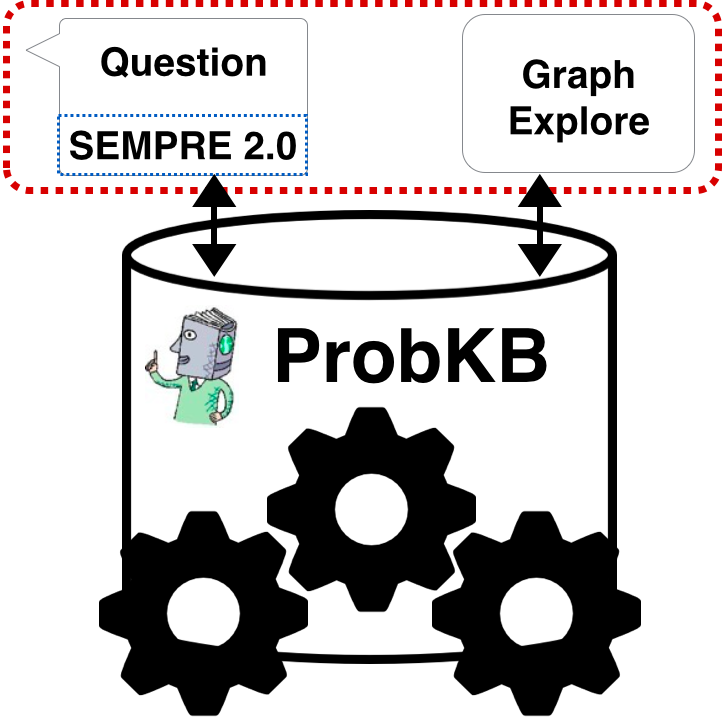
\includegraphics[width=\columnwidth,clip=true,trim=0cm 4cm 0cm 10cm]{images/qaarchitecture.png}
\caption{Question Answering system architecture.}
\label{fig:qaarchitecture}
\end{figure}



This demonstration describes a question answering systems designed around
a probabilistic knowledge base.
In this section, describe each component of the knowledge base system.
We begin with the interface, we describe each of the different methods
the users has to interact with with the backend knoweldge base.
We then describe the Logic layer that does translation and of user actions
to the back end actions. It also allows the user to see the current current
status of the system.
We also describe the probabilistic knowledge base driving the system.
We describe its schema and the integrated functions.



\subsection{Interface}

The framework is developed using AngularJS\@ to completely compatible with desktop and mobile devices.
The interface allows users to make queries using three different modalities.
Users will be able to enter natural language questions, search through the set of existing facts, and use a graph to explore connections between graphs.
New probabilistic facts and rules can also be added to the system through the interface.
Users can also remove or alter the existing facts and rerun queries.
The status of queries and the underlying processes are displayed on the main interface.


\subsubsection{Natural Language Interface}
Describe the purpose tranlation of natual language questions queries.
Add the auto complete for previous questions.

%QUEPY

%SEMPRE
We create a service that calls the SEMPRE 1.0 question answering system~\cite{berant2013freebase,berant2013semantic}.
This service takes a natural language questions matches against predicates aligned with Freebase.
We are then able to generate SPARQL queries to determine the answer of a query.



\subsubsection{Fact Search}
Describe how facts are searched using the database.
Describe how results are ranked.
Describe how new results are discovered.
\subsubsection{Graph Exploring}
Describe D3 visualization of graph and rule display
Describe user interaction with graph
Describe user selecting facts
Describe users removing facts


\subsection{Logic}
Describe the translation of NL-to-queries using templates (quepy) and also sempre.

Describe how rankings are computed from queries.
SEMPRE Returns probabilities, Quepy gives a 0 or 1 probability.
We compare the fact pobabilities to the sempre results.

\subsection{Knowledge Base}

Desscribe the PostgreSQL database and the other serices running on servers.
Describe the tables 
Describe the functions that are called
Describe the parallelism

The system is loaded with docker, a system container, so any modifications by demo can be quickly rolled back to the intial state.





% See other examples: http://www.vldb.org/2014/program/papers/demo/





\section{Related Work}

Several existing research projects have aimed to extract answers from knowledge bases~\cite{yahya2012natural,yao2014information}.
In this work, we leverage existing research to demonstrate the utility of probabilistic knowledge bases.
Previous methods rank answers by their compatibility to the question.
We additionally compute the joint probability of the underlying facts, providing an additional dimension to the answer.
Furthermore, previous works only use deterministic rules, so they are not able to extract a similar confidence score.

% http://nakashole.com/papers/2012-vlds-urdf.pdf
Nakashole and Mitchell~\cite{nakashole2014languageaware} describe a system,
FactChecker, that discovers whether facts are believable by observing the
semantics and considering alternatives. 
In this work, we only use knowledge bases and have no access to the source
knowledge accuracy of the extractions and context.
Such a constraint also separates this work from knowledge bases such as
Knowledge Vault~\cite{dong2014knowledge} that require source information in
response to a user search.



\section{Demonstration Plan}

\begin{figure*}
\centering
 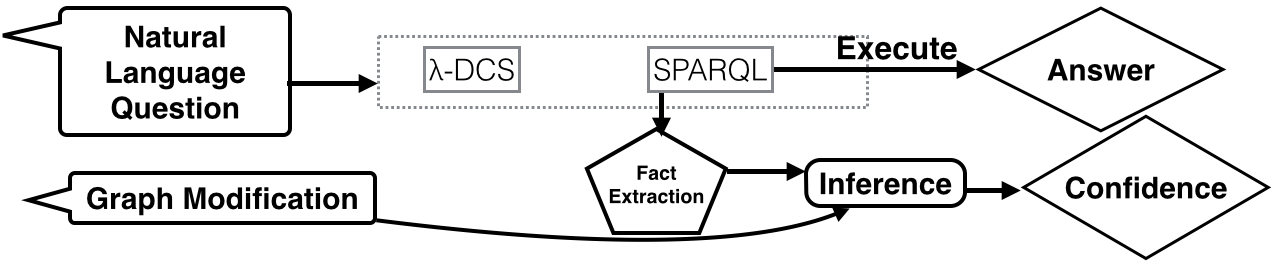
\includegraphics[width=0.9\linewidth]{images/probqa-pipeline.png}
 \caption{Probabilistic knowledge base assisted question answering demonstration pipeline.}
\label{fig:probqa-pipeline}
\end{figure*}


During the demo, attendees will be given the work flow shown in Figure~\ref{fig:probqa-pipeline}.
An attendee may submit a natural language question to the interface of retrieve one of the pre-seeded utterances.
This question is then translated to the \(\lambda\)-DCS and SPARQL using the SEMPRE system.
The user is then shown the answer to the question, as computed by the SPARQL
query and also the truthfulness result of the answer.

Alternatively, an attendee may interact with the knowledge base through a graphical interface.
Attendees will be able to search through the set of existing facts or use a graph to explore connections between graphs.
New probabilistic facts and rules can also be added to the system through the interface.
Users can also remove or alter the existing facts and rerun queries or answer more questions.
The status of queries and the underlying processes are displayed on the main interface.




%We can visualize the ranking of candidates with each candidates truthfulness value.

%Describe D3 visualization of graph and rule display
%Describe user interaction with graph
%Describe user selecting facts
%Describe users removing facts

%Features
%  Add the auto complete for previous questions.

%Describe how users will be able to alter parameters.


The demo application is developed using AngularJS\@ to be completely compatible with desktop and mobile devices.
We also load the data sets described in Section~\ref{sec:probqa-dataset} into a PostgreSQL DBMS\@.
We train SEMPRE models for question answering on each of the three knowledge bases.
We translate the SPARQL queries to relational format using OpenRDF and Apache Jena SDB\@.
%Describe the tables 
%Describe the functions that are called
%Describe the parallelism
We install the database and web server on docker system container, so any modifications by demo can be quickly rolled back to the initial state.







\balance

\section{Acknowledgments}
This work was partially supported by DARPA under FA8750-12-2-0348-2
(DEFT/CUBISM) and Christan Grant was supported by a NSF Graduate Research
Fellowship, Grant DGE-0802270.



\bibliographystyle{abbrv}
\bibliography{citations}  % vldb_sample.bib is the name of the Bibliography in this case


\end{document}




